% chapter 4 section 3

\section{磁场}

\subsection{磁场}

\subsubsection{电与磁}

磁的体系与电十分类似,几乎所有磁的概念\footnote{磁场中不存在独立的单极磁荷}都可以在电中找到对应的内容。
\begin{figure}[ht!]
    \centering
    \renewcommand\arraystretch{1.2}
    \begin{tabular}{c|c|c}
        \hline
        &电&磁\\\hline
        基本单位&电荷C&磁荷Wb\\\hline
        场力&电场力(库仑力)&磁场力\\\hline
        场常数&电容率$\varepsilon$(誘電率)&磁导率$\mu$(透磁率)\\\hline
    \end{tabular}
    \caption{电与磁对比}
\end{figure}

因此,磁场的直觉定义即为
\begin{equation*}
    \vec{H}=\frac{\vec{F}}{m}\quad(N/Wb)
\end{equation*}
同样也存在描述磁场走势、大小等信息的磁场线,并具有以下性质。
\begin{itemize}
    \item N极出,S极入
    \item 磁场线密$\iff$磁场强
\end{itemize}
\begin{figure}[ht!]
    \centering
    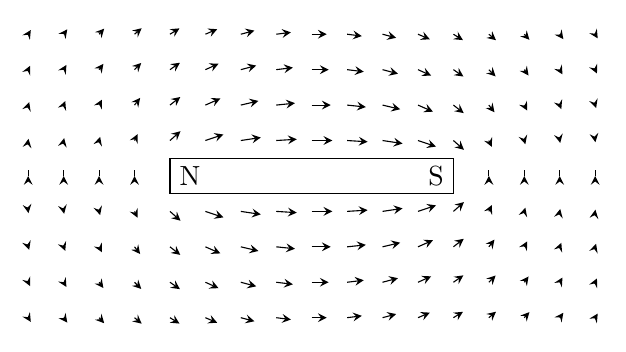
\begin{tikzpicture}[scale=0.45]
        \foreach \x in {-8,...,8} \foreach \y in {-4,...,4} {
            \pgfmathparse{or(
                and(equal(\x,-4),equal(\y,0)),
                and(equal(\x,4),equal(\y,0))
            )}
            \ifnum\pgfmathresult=1
            \else
            \draw[-stealth] (\x,\y) -- ++ (
                {0.3*((\x+4)/sqrt((\x+4)^2+(\y)^2)-(\x-4)/sqrt((\x-4)^2+(\y)^2))},
                {0.3*(\y/sqrt((\x+4)^2+(\y)^2)-\y/sqrt((\x-4)^2+(\y)^2))}
            );
            \fi
        }
        \filldraw[color=black, fill=white] (-4,-0.5) -- node[right] {N} (-4,0.5) -- (4,0.5) -- node[left] {S} (4,-0.5) -- cycle;
    \end{tikzpicture}
    \caption{磁场图示}
\end{figure}

\subsubsection{电生磁}

19世纪初叶,毕奥-萨伐尔定律\footnote{
    Biot-Savart Law
    \begin{equation*}
        \mathbf{B}=\frac{\mu_0}{4\pi}\int\mathbf{J}\times\frac{\mathbf{r}-\mathbf{l}}{|\mathbf{r}-\mathbf{l}|^3}d^3l
    \end{equation*}
}、安培定律\footnote{
    Ampère's circuital law
    \begin{equation*}
        \oint_{\partial S}\mathbf{B}\cdot d\mathbf{l}=\mu_0\int_S\mathbf{J}\cdot d\mathbf{S}
    \end{equation*}
}等揭示了电流的磁作用,其中以下三种模型十分具有代表性。
\begin{figure}[ht!]
    \centering
    \begin{minipage}[t]{0.48\textwidth}
        \centering
        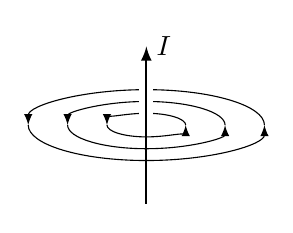
\begin{tikzpicture}
            \foreach \r in {0.5,1,1.5} {
                \draw[-latex] (\r,0) arc (0:180:{\r} and {\r*0.3});
                \draw[-latex] ({-\r},0) arc (-180:0:{\r} and {\r*0.3});
            }
            \draw[color=white, line width=5pt] (0,0) -- (0,1);
            \draw[thick, -latex] (0,-1) -- (0,1) node[right] {$I$};
        \end{tikzpicture}
        \caption{直线电流磁场}
    \end{minipage}
    \begin{minipage}[t]{0.48\textwidth}
        \centering
        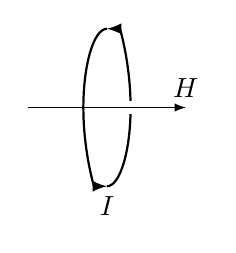
\begin{tikzpicture}
            \draw[thick, -latex] (0,-1) arc (-90:90:0.3 and 1);
            \draw[color=white, line width=5pt] (0,0) -- (1,0);
            \draw[-latex] (-1,0) -- (1,0) node[above] {$H$};
            \draw[thick, -latex] (0,1) arc (90:270:0.3 and 1) node[below] {$I$};
        \end{tikzpicture}
        \caption{环形电流磁场}
    \end{minipage}
    \begin{minipage}{\textwidth}
        \centering
        \begin{tikzpicture}
            \clip (-0.5,-1) rectangle (4,1);
            \draw[thick, midarrow] (0,-1) -- node[left] {$I$} (0,0);
            \draw[thick] (0,0) arc (180:135:0.2 and 0.4);
            \draw[color=white, line width=5pt] (-0.5,0) -- (0.2,0);
            \draw[-latex] (-0.5,0) -- (3.5,0) node[above] {$H$};
            \foreach \n in {0,...,5} {
                \draw[color=white, line width=5pt] ($(0.2+\n*0.4,0)+(135:0.2 and 0.4)$) arc (135:-135:0.2 and 0.4);
                \draw[thick, midarrow] ($(0.2+\n*0.4,0)+(135:0.2 and 0.4)$) arc (135:-135:0.2 and 0.4);
            }
            \draw[color=white, line width=5pt] (2.8,0.2) -- (2.8,-1);
            \draw[thick] ($(2.6,0)+(135:0.2 and 0.4)$) arc (135:0:0.2 and 0.4);
            \draw[thick,midarrow] (2.8,0) -- (2.8,-1);
        \end{tikzpicture}
        \caption{线圈周围磁场}
    \end{minipage}    
\end{figure}
\begin{itembox}[l]{电流产生的磁场}
    \begin{itemize}
        \item 直线电流
        \begin{equation*}
            H=\frac{I}{2\pi r}
        \end{equation*}
        \item 环形电流(中心处)
        \begin{equation*}
            H=\frac{I}{2r}
        \end{equation*}
        \item 线圈
        \begin{equation*}
            H=nl\quad(n:\textrm{线圈匝数})
        \end{equation*}
    \end{itemize}
\end{itembox}

\subsection{安培力}

\textbackslash\textbackslash TODO

\subsection{洛伦兹力}

\textbackslash\textbackslash TODO
